\documentclass[12pt,letterpaper]{article}
\usepackage[utf8]{inputenc}
\usepackage[english]{babel}
\usepackage{amsmath}
\usepackage{amsfonts}
\usepackage{amssymb}
\usepackage{graphicx}
\usepackage{units}

%%%%
\usepackage{multicol}
\usepackage{lscape}
%%%%

\usepackage{hyperref}
\usepackage{booktabs} % Allows the use of \toprule, \midrule and \bottomrule in tables
\newcommand\Fontvi{\fontsize{9}{6.2}\selectfont}
\usepackage{float}
\usepackage{subfig}
%\usepackage[spanish, activeacute]{babel}
\usepackage{filecontents,hyperref,listings}
\usepackage[round]{natbib}
\usepackage{ragged2e} %these packages allow paragraph alignment 
\usepackage{etoolbox}
\apptocmd{\frame}{}{\justifying}{} % Allow optional arguments after frame.
\usepackage[ruled]{algorithm2e}
\graphicspath{{img/}} % this command is to add the figure path
%%

\usepackage[left=2cm,right=2cm,top=2cm,bottom=2cm]{geometry}
\author{Juan Gomez}
\usepackage{cleveref}
\crefname{equation}{eq.}{eqs.}
\crefname{algorithm}{alg.}{algs.}
\author{Área de Mecánica Computacional}
\title{\textbf{Convergence of analysis results}}
%
\begin{document}
\maketitle

\section{Cantilever beam}
\Cref{fig:viga} shows a cantelever beam under a tip load $P$. The beam is of length $l$; moment of inertia $I$; height $2c$ and material properties corresponding to Poissons ratio and Young modulos $\nu$ and $E$ respectively.

\begin{figure}[H]
\centering
\subfloat{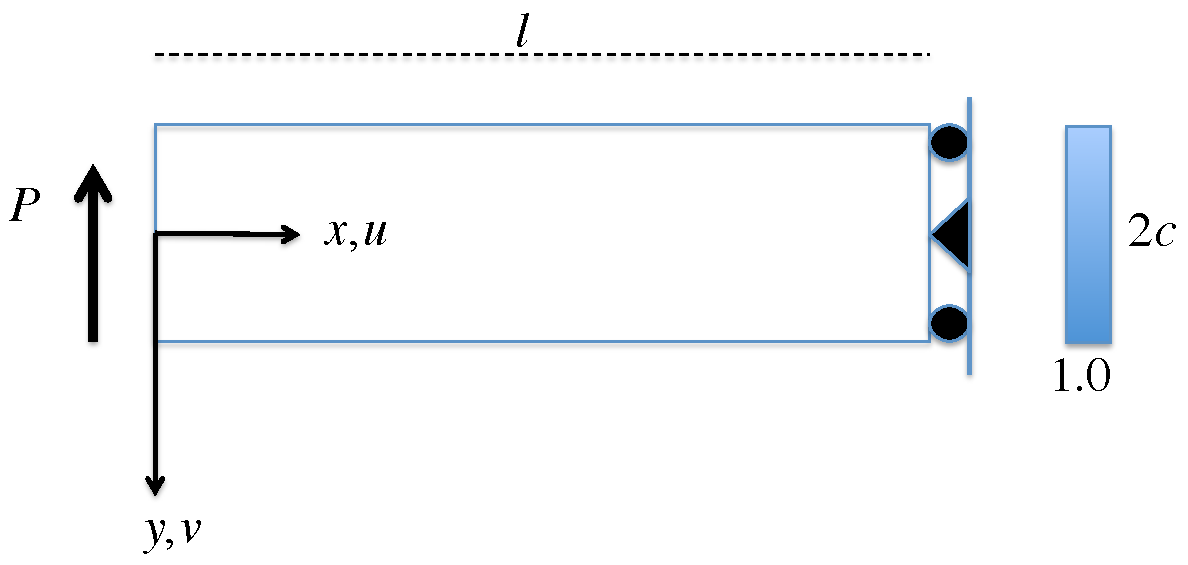
\includegraphics[width=0.75\textwidth]{img/beam.pdf}}
\caption{Cantelever beam.}
\label{fig:viga}
\end{figure}

The analytic solution \citep{book:timoshenko} is given by:

\[u =  - \frac{P}{{2EI}}{x^2}y - \frac{{\nu P}}{{6EI}}{y^3} + \frac{P}{{2IG}}{y^3} + \left( {\frac{{P{l^2}}}{{2EI}} - \frac{{P{c^2}}}{{2IG}}} \right)y\]

\[v = \frac{{\nu P}}{{2EI}}x{y^2} + \frac{P}{{6EI}}{x^3} - \frac{{P{l^2}}}{{2EI}}x + \frac{{P{l^3}}}{{3EI}}\]

\[{\varepsilon _{xx}} = \frac{{\partial u}}{{\partial x}} \equiv  - \frac{P}{{EI}}xy\]

\[{\varepsilon _{yy}} = \frac{{\partial v}}{{\partial y}} \equiv \frac{{\nu P}}{{EI}}xy\]

\[{\gamma _{xy}} = \frac{{\partial u}}{{\partial y}} + \frac{{\partial v}}{{\partial x}} \equiv \frac{P}{{2IG}}\left( {{y^2} - {c^2}} \right)\]

while the particular solution for parameters $E=1000.0$, $\nu=0.30$, $l=24$ and $2c=8$ is shwon below:

\begin{figure}[H]
\centering
\subfloat{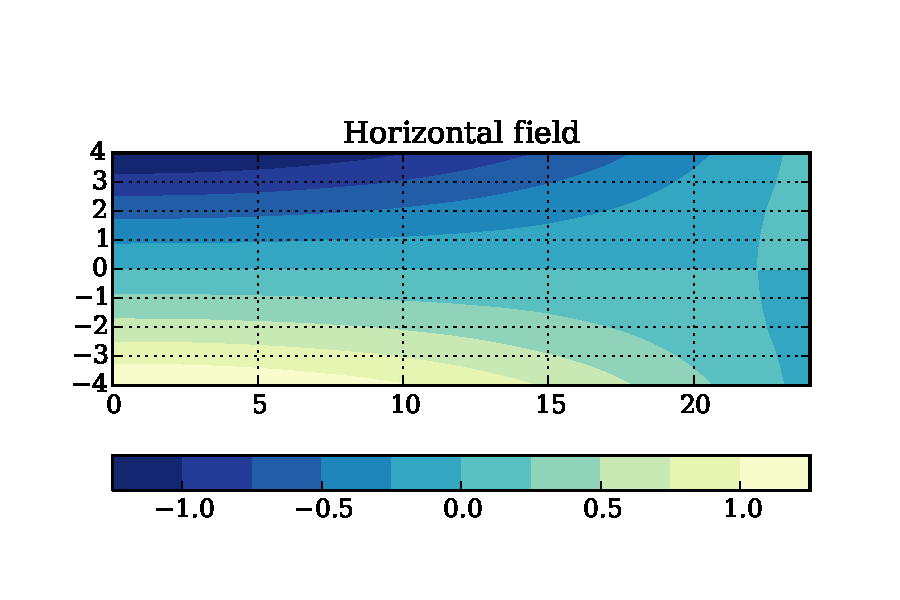
\includegraphics[width=0.75\textwidth]{img/anahorizo.pdf}}//
\subfloat{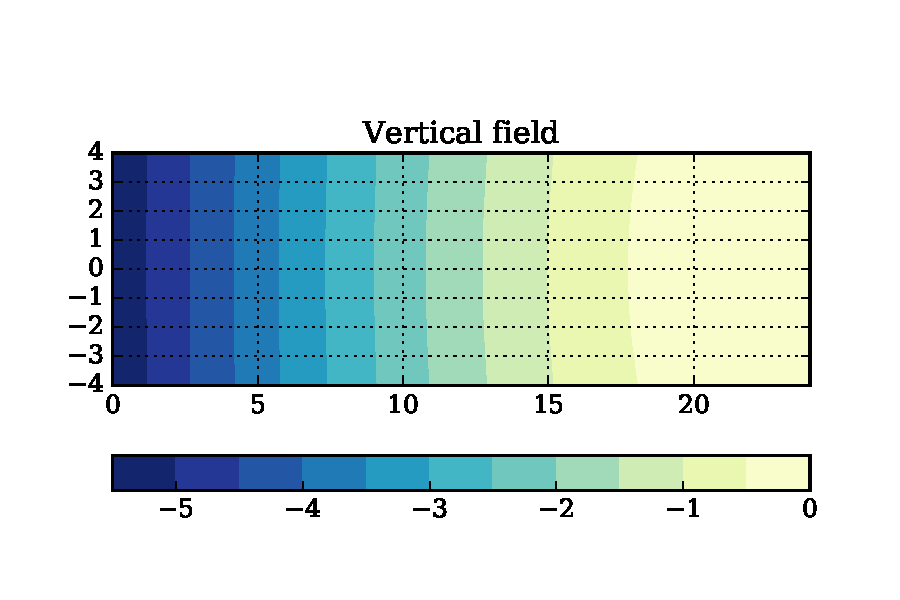
\includegraphics[width=0.75\textwidth]{img/anavertic.pdf}}
\caption{Horizontal field.}
\label{fig:ecuacion}
\end{figure}

The beam was also analyzed with the FEM using solid lineal square elements under plane stress conditions. We conducted $5$ different analysis with the following set of characteristic element size $h=[6.0,3.0,1.5,1.0,0.5]$. The meshes are shown in \cref{fig:mallas}

\begin{figure}[H]
\centering
\subfloat{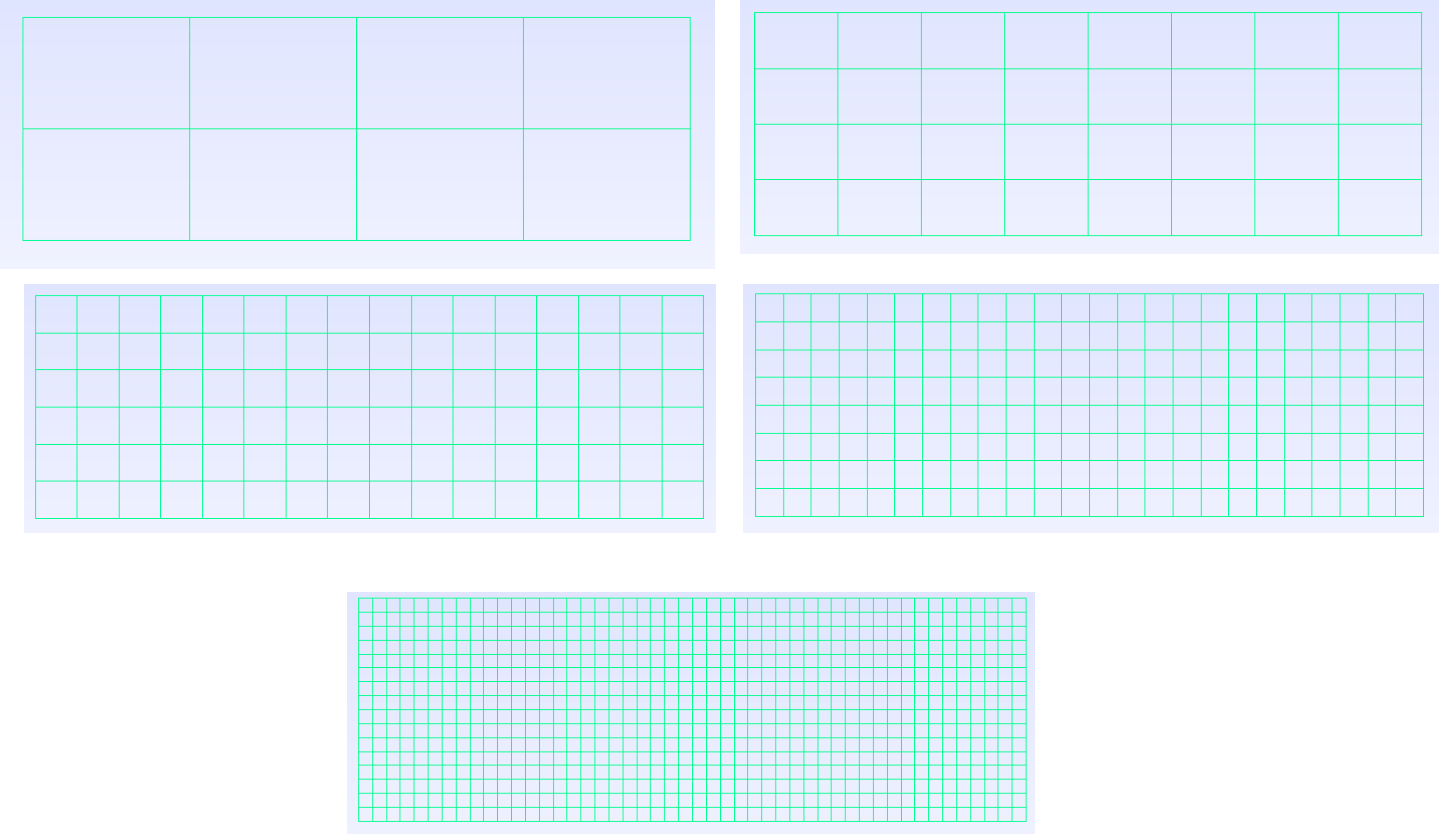
\includegraphics[width=0.75\textwidth]{img/meshes.pdf}}
\caption{Finite element meshes.}
\label{fig:mallas}
\end{figure}

The horizontal and vertical displacement contours for the FE-solution and the analytic solution are compared in \cref{fig:sls} for the case $h=1.0$. Notice that in the finite elment models the load is applied as nodal point loads of the same magnitud distributed along all the nodes at $x=0$. This implies a uniform load distribution instead of the parabolic load consitent with the shear stress in the analytic solution.

\begin{figure}[H]
\centering
\subfloat{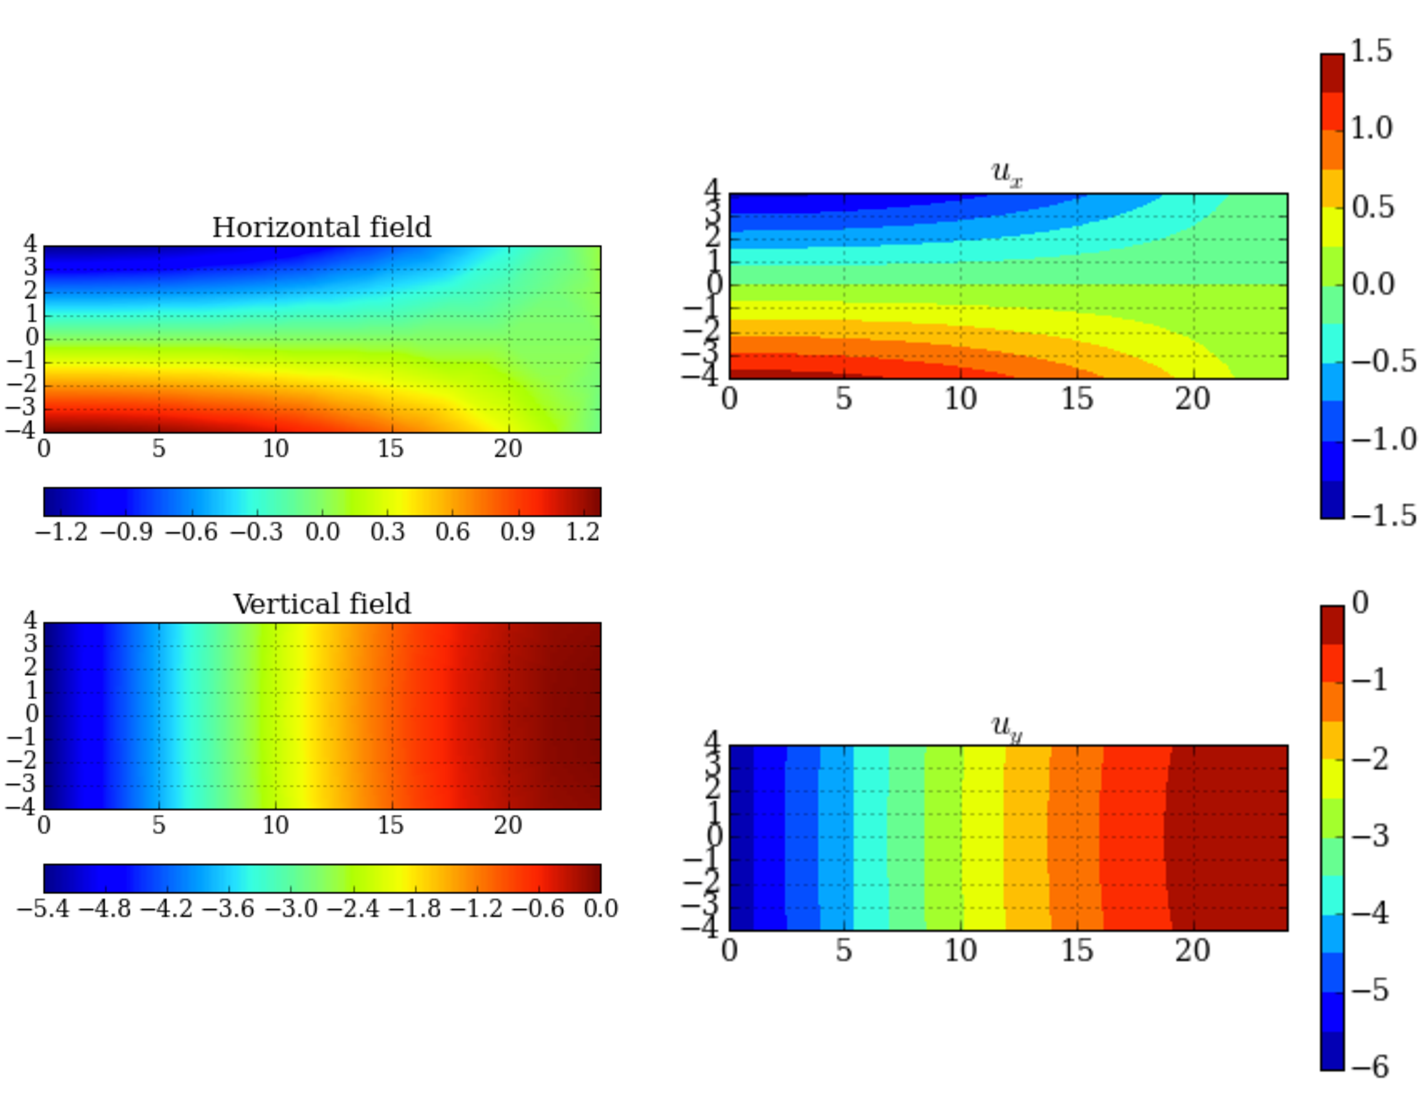
\includegraphics[width=0.75\textwidth]{img/compara.pdf}}
\caption{Analytic (left) vs Numerical (right) solution.}
\label{fig:sls}
\end{figure}

\[{\prod _{FE}} =  - \frac{1}{2}{U^T}KU\]

\[{\prod _{Exa}} = \frac{{\prod _{n - 1}^2 - {\prod _n}{\prod _{n - 2}}}}{{2{\prod _{n - 1}} - {\prod _n} - {\prod _{n - 2}}}}\]

Using $n=5$ we have ${\prod _{Exa}}=-154.09$.

\[\left\| {{{\vec u}_{Exa}} - {{\vec u}_{FE}}} \right\| \equiv {({\prod _{Exa}} - {\prod _{FE}})^{1/2}}\]


\begin{center}
\begin{tabular}{ |c|c|c|c| }
  \hline
  $h$ & ${\prod _{FE}}$ & $\left\| {{{\vec u}_{Exa}} - {{\vec u}_{FE}}} \right\|$ & $\frac{{\left\| {{{\vec u}_{Exa}} - {{\vec u}_{FE}}} \right\|}}{{\left\| {{{\vec u}_{Exa}}} \right\|}}$ \\
  \hline 
  $6.0$  & $-118.414$ & $5.973$  & $0.481$  \\
  \hline
   $3.0$  & $-139.273$ & $3.849$  & $0.310$  \\
  \hline
   $1.5$  & $-145.866$ & $2.868$  & $0.231$  \\
  \hline
   $ 1.0$  & $-147.501$ & $2.567$  & $0.207$  \\
  \hline
  $ 0.5$  & $-148.811$ & $2.298$  & $0.185$  \\
  \hline
\end{tabular}
\captionof{table}{Convergence of anlysis results}
\label{ejemplo}
\end{center}

\begin{figure}[H]
\centering
\subfloat{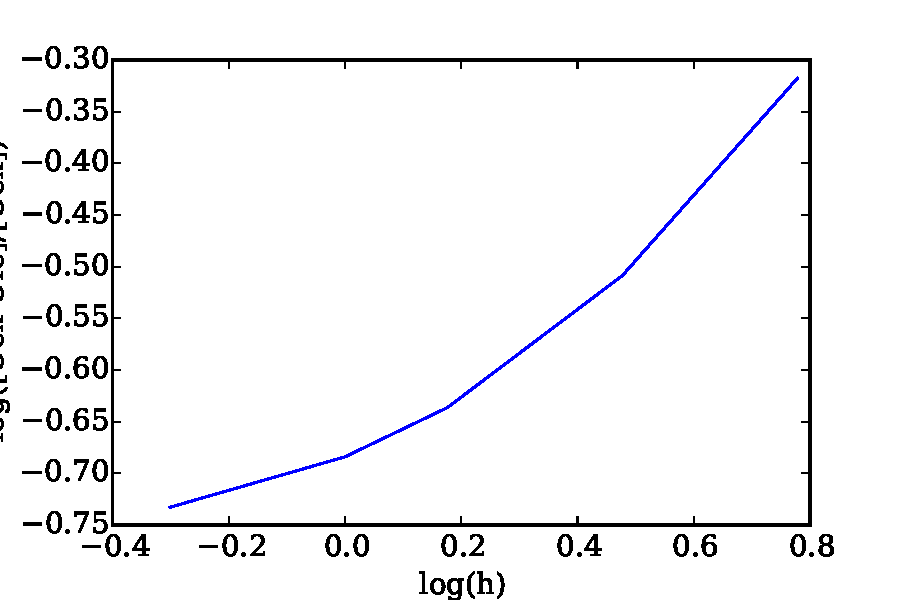
\includegraphics[width=0.65\textwidth]{img/conver.pdf}}
\caption{Energy norm of the error}
\label{fig:conv}
\end{figure}

\[\log \left( {\left\| {{{\vec u}_{Exa}} - {{\vec u}_{FE}}} \right\|} \right) = \log c + k\log h\]




\bibliographystyle{gji}
\bibliography{references}





\end{document}